\documentclass[11pt]{article}
\usepackage{hyperref}
\usepackage[spanish]{babel}
\usepackage[utf8]{inputenc}
\usepackage{pdfpages}
\usepackage[bottom=8em]{geometry}
\usepackage{amsmath}
\usepackage{mathtools}
\usepackage{pdflscape}
\usepackage{float}
\usepackage{mathtools}
\usepackage{booktabs}
\usepackage{layout}
\usepackage{soul}

\begin{document}

%%%%%%%%%%%%% COVER %%%%%%%%%%%%%%%%
\begin{titlepage}
\begin{center}
\begin{tabular}[c]{c c}
\begin{tabular}[b]{l}
\Huge
\textsf{UNIVERSIDAD POLITÉCNICA DE MADRID}
\end{tabular}
\\
\end{tabular}

\vspace{0.9cm}

\Large
\textsf{\textbf{ESCUELA TÉCNICA SUPERIOR DE INGENIERÍA DE SISTEMAS INFORMÁTICOS}}

\vspace{0.5 cm}

\Large
Título de Experto en Arquitectura y Desarrollo Software


\includegraphics[scale=1]{img/logo_etsisi.png}

\vspace{0.9cm}

\Huge
PROYECTO FIN DE EXPERTURÍA

\vspace{0.9cm}

\Large
\textbf{Medición de calidad de código en proyectos Open Source en base a métricas}

\vspace{0.7cm}

\Large
Autor: Sergio Arroutbi Braojos \\
Tutor: Micael Gallego Carrillo

\vspace{0.5cm}

Febrero de 2016

\vspace{0.9cm}
\begin{tabular}[c]{c c}
\begin{tabular}[b]{l}
\Huge
\textsf{UNIVERSIDAD POLITÉCNICA DE MADRID} \\
\end{tabular}
\\
\end{tabular}

\vspace{1cm}

\Large
\textsf{\textbf{ESCUELA TÉCNICA SUPERIOR DE INGENIERÍA DE SISTEMAS INFORMÁTICOS}}

\end{center}
\end{titlepage}
%%%%%%%%%%%%%%%%%%%%%%%%%%%%%%%%%%%%%%



\renewcommand{\listtablename}{Lista de Tablas}
\renewcommand{\tablename}{TABLA} 

\hypersetup
{   
pdfborder={0 0 0}
}
   
\pagebreak

\tableofcontents
\listoftables
\listoffigures

\pagebreak

\section{Introducción}

Este documento es una aproximación al mundo de la calidad en el software y, más en concreto, en el código Open Source. La calidad del software es medible, así como también lo es el código fuente que permite construir dicho software. Se define como calidad del software al campo de estudio que describe aquellos atributos de los productos software que son deseables.

Para medir la calidad del código fuente, la utilización de las métricas es fundamental. Se conoce como métrica de software a aquella medida cuantitativa que permite conocer en qué grado un sistema, componente o proceso cumple un atributo determinado~\cite{ieeeglossary:softwareengineeringterminology}.

Las métricas se han convertido en un ornamento más dentro de las suites de herramientas de gestión del ciclo de vida de desarrollo, proporcionando de un solo vistazo la salud del proyecto a través de paneles de métricas.
El principal problema viene a la hora de conocer qué métricas son más importantes, cuáles lo son menos, cuáles deben tener un seguimiento diario, etc.~\cite{abistock:usingmetrics}

Dicho lo anterior, cabe destacar que en los proyectos Open Source, la propia naturaleza del código fuente, que debe ser accesible de forma pública y usable sin restricciones, hace que la calidad de éste sea aún más importante. El software Open Source es, por su naturaleza, transparencia, y la calidad del código fuente no impacta únicamente en los desarrolladores, sino que es a su vez un factor directamente visible para los potenciales usuarios.
La pretensión de este documento es, en la medida de lo posible, y de forma gradual, describir y detallar una serie de métricas que puedan obtenerse a través de las herramientas disponibles de forma que permitan especificar un modelo de calidad en base a dichas métricas.

\subsection{Objetivos}
A continuación se definen los objetivos de este trabajo:
\begin{itemize}
\item{El objetivo de este documento es, en primer lugar, enumerar la existencia de algunos modelos de calidad en el software de tipo Open Source, exponiendo qué carencias muestran a la hora de analizar el código fuente}.
\item{Tras ello, se propondrá la definición de un modelo de calidad propio que establezca métricas de análisis de código fuente que permitan comparar la calidad de proyectos Open Source y permita ponderar cada una de ellas en la evaluación del resultado final. La principal idea no es llegar a un método extremadamente eficiente o exhaustivo, sino más bien justificar la selección y ponderación de las diversas métricas en base a determinados criterios, de forma que se llegue a la personalización de un modelo de calidad propio para el código fuente. Esto permitirá, además, realizar un repaso por los conceptos más importantes relacionados con el diseño orientado a objetos (acoplamiento, cohesión, encapsulación, modularidad, jerarquía, herencia, etc.)}.
\item{Por otro lado, se realizará el estudio, integración e implementación de las herramientas que permitan aglutinar las métricas definidas, así como ponderar cada una de las mismas, para llegar a una evaluación final. Se evaluarán las herramientas existentes en el estado del arte, se realizarán los pasos que permitan integrarlas entre sí y se implementará un mecanismo que permita su ejecución y sincronización. Se contemplarán, además, aquellas limitaciones existentes, cómo afectan al modelo de calidad establecido y, en qué forma, se podría modificar el modelo para ajustarlo a las herramientas disponibles y al estado del arte de las mismas}.
\item{Finalmente, se realizará un ejemplo práctico de análisis de proyectos Open Source, de forma que se muestre la aplicación del método a través de las herramientas estudiadas para su comparativa. Así, se expondrá la comparativa entre diversos proyectos, de forma que se evalúen dos proyectos de similares características. Por otro lado, se establecerá el análisis para dos versiones de un mismo proyecto. Esto permitirá conocer la evolución de la calidad de un proyecto Open Source en el tiempo}.
\end{itemize}

\subsection{Estructura del documento}
Para acometer los objetivos previamente descritos, este documento sigue la siguiente estructura:

\begin{enumerate}
\item{\underline{Introducción}}. Se establecerá una introducción con un resumen de los contenidos del documento. Así se enumerarán en este apartado la misión del trabajo, los objetivos que éste pretende así como la estructura del presente documento.
\item{\underline{Modelos de Calidad}}. Como primera aproximación, en este apartado se introducirán los modelos de calidad ya existentes para proyectos Open Source, como OpenBRR, QSOS o QualOSS. Estos modelos, sin embargo, no realizan un análisis avanzado del estado del código y la calidad del mismo, si bien sí que analizan aspectos relacionados con la calidad del código, al menos, indirectamente, como el número de BUGS.
Hilando con esto, se enumerarán distintas métricas que son importantes a la hora de establecer calidad en el software, como por ejemplo desde el número de métodos por clase, número de atributos por clase, dependencias con otras clases, número de parámetros por método o complejidad ciclomática.
Finalmente, en este apartado se describirán las características que un modelo de calidad basado en métricas software del estilo de OpenBRR pero enfocado única y exclusivamente al análisis de éstas últimas, con una ponderación que permita establecer la calidad y una justificación de la misma, en cuanto a qué métricas son consideradas más importantes y por qué.
\item{\underline{Herramientas}}. En este apartado se describirán aquellas herramientas que permiten obtener una o varias de las métricas anteriores, y cómo se pueden combinar dichas herramientas para llegar a la evaluación de calidad final. Se contemplarán, igualmente, herramientas de desarrollo propio o adaptaciones a herramientas ya existentes. 
Además, se mostrarán diversas gráficas y/o reportes comparativos de la calidad del código para un determinado proyecto. Así, se podrá mostrar de forma gráfica una comparativa de aquellas métricas más determinantes del sujeto a analizar.
Este apartado permitirá ver el estado del arte de las herramientas de análisis de métricas para, de esta forma, empezar a establecer cuáles de ellas se van a utilizar a la hora de establecer el modelo de calidad propuesto.
\item{\underline{Propuesta de un modelo de calidad}}. Esta sección permitirá establecer, en base a los dos capítulos anteriores, un modelo de calidad de software orientado a métricas. De esta forma se elaborará un modelo, iterativo e incremental, que permitirá establecer las métricas a evaluar, las herramientas que permitan dicha evaluación y la ponderación de cada una de las métricas y/o grupos de métricas.
\item{\underline{Caso práctico: MongoDB vs. RethinkDB vs. ArangoDB}}. En este apartado se realizará el análisis de dos o más proyectos Open Source, de un tamaño similar en líneas de código, escritos en C++. De esta forma, se podrán concretar los aspectos vistos anteriormente en una comparativa real.
En concreto, se realizará la comparativa entre bases de datos NoSQL escritas en C++, como son MongoDB, RethinkDB y ArangoDB.
\item{\underline{Evaluación de histórico de calidad en el tiempo}}. En este apartado se detallará la evaluación de los proyectos anteriormente descritos en un período de tiempo determinado, con el fin de conocer cómo ha sido dicha evolución en función del modelo de calidad planteado.
\item{\underline{Mejoras y posibles trabajos futuros}}. Finalmente, dentro de esta sección, se recogerán mejoras y posibles trabajos futuros que se podrían realizar para mejorar o extender lo que se haya realizado en este proyecto. Se contemplarán, por tanto, opciones de extender el modelo de calidad con más métricas, o bien incluir aspectos que no se han contemplado, extender el modelo para más lenguajes de programación, etc.
\end{enumerate}

\pagebreak

\section{Modelos de Calidad}
En esta sección se pretende llegar a un modelo de calidad, basado en métricas, que permita realizar la comparación entre dos o más proyectos Open Source, o el estado de uno proyecto a lo largo del tiempo. Así, se estudiará el estado del arte de los modelos de calidad en proyectos Open Source más utilizados en la actualidad, para ver si se pueden utilizar en su totalidad, o, al menos, de forma parcial.

Por otro lado, se establecerán diversas métricas que son consideradas en la medición de la calidad de software, tanto desde el punto de vista de programación funcional, como, sobre todo, en el software diseñado en base a orientación a objetos. Además de enumerar las métricas más importantes, se realizará la categorización y priorización de las mismas. Esto permitirá establecer un modelo de calidad en base a métricas según la categorización establecida.

\subsection{Modelos de calidad en proyectos Open Source}

Si bien a veces, aunque cada vez menos, los proyectos Open Source se consideran caóticos, no robustos, que no son utilizados por grandes compañías de software o que son, por naturaleza, proyectos que no disponen de soporte, está más que justificado que estas aseveraciones no son más que mitos en torno a este tipo de software~\cite{oreilly:tenmythsaboutopensourcesoftware}.

El software Open Source, por estar más expuesto, posee igual o mejor calidad que el software privativo. Además, existen diversos modelos de calidad que permiten establecer la calidad de un proyecto Open Source, y sobre todo comparar la calidad contra otro proyecto de forma que el usuario disponga de información para decantarse en caso de que se tenga que tomar una decisión sobre el proyecto que se va a utilizar.

Obviamente, si bien los usuarios finales particulares no someten el software a un modelo de calidad para decantarse por un software de tipo Open Source u otro, y se basan más en una evaluación menos procedimental y más orientada a experiencia de usuario (basada en facilidad de uso, funcionalidad, etc.), sí que es cada vez más común, en el ámbito empresarial, enfrentar varios proyectos Open Source a un modelo de calidad establecido o bien a un modelo de calidad adaptado a las necesidades de la empresa para tomar la decisión de la adquisición final.

Si bien los objetivos de este documento no son realizar un estudio detallado de los modelos de calidad existentes en el software Open Source, sí que resulta interesante presentar dichos modelos para ver qué ofrecen, qué aspectos consideran importantes y qué tipo de evaluación llevan a cabo para establecer sus criterios de calidad.

Antes de hablar de los modelos existentes, cabe destacar que existen dos tipos de modelos de calidad a la hora de evaluar proyectos Open Source:

\begin{itemize}
\item{\underline{Modelos de calidad ligeros}}. Este tipo de modelos son de una implementación más ligera y sencilla respecto a los pesados. Ejemplos de este tipo de modelo son OpenBRR y QSoS.
\item{\underline{Modelos de calidad pesados}}. Este tipo de modelos, de mayor complejidad y dificultad en su implementación, son considerados más exactos en cuanto a la extensión de su estudio en torno al software. El modelo de calidad de este tipo más conocido es QualOSS.
\end{itemize}

\subsubsection{Modelos Ligeros de Análisis de Calidad de proyectos Open Source}

Como ya se expuso anteriormente, este tipo de modelos son de sencilla implementación. Así, establecer la calidad de un proyecto Open Source puede llegar a ser tan sencillo como rellenar una hoja de cálculo con diversas preguntas y ponderar los resultados resultantes. Éste el es caso de OpenBRR.

\begin{itemize}
\item{\underline{OpenBRR}} (Open Business Readiness Rating). Pese a que en la actualidad se está migrando a un modelo más evolucionado, conocido como OSSpal~\cite{osspal:osspal}, este modelo de calidad ha sido, sin duda, el más sencillo de implementar de los existentes en la actualidad. Como ya se ha comentado, básicamente es una hoja de cálculo que define una serie de super-atributos (conocidos también en el modelo como categorías), con una serie de subcategorías, que no son más que métricas aplicadas a cada una de las categorías. El usuario puede establecer diferentes pesos tanto a las categorías como a las subcategorías. El modelo establece, finalmente, la puntuación final en función de los pesos asignados por el usuario. En la siguiente figura se muestra una de las múltiples categorías del modelo:

\begin{center}
 \begin{figure}[H]
 \begin{center}
   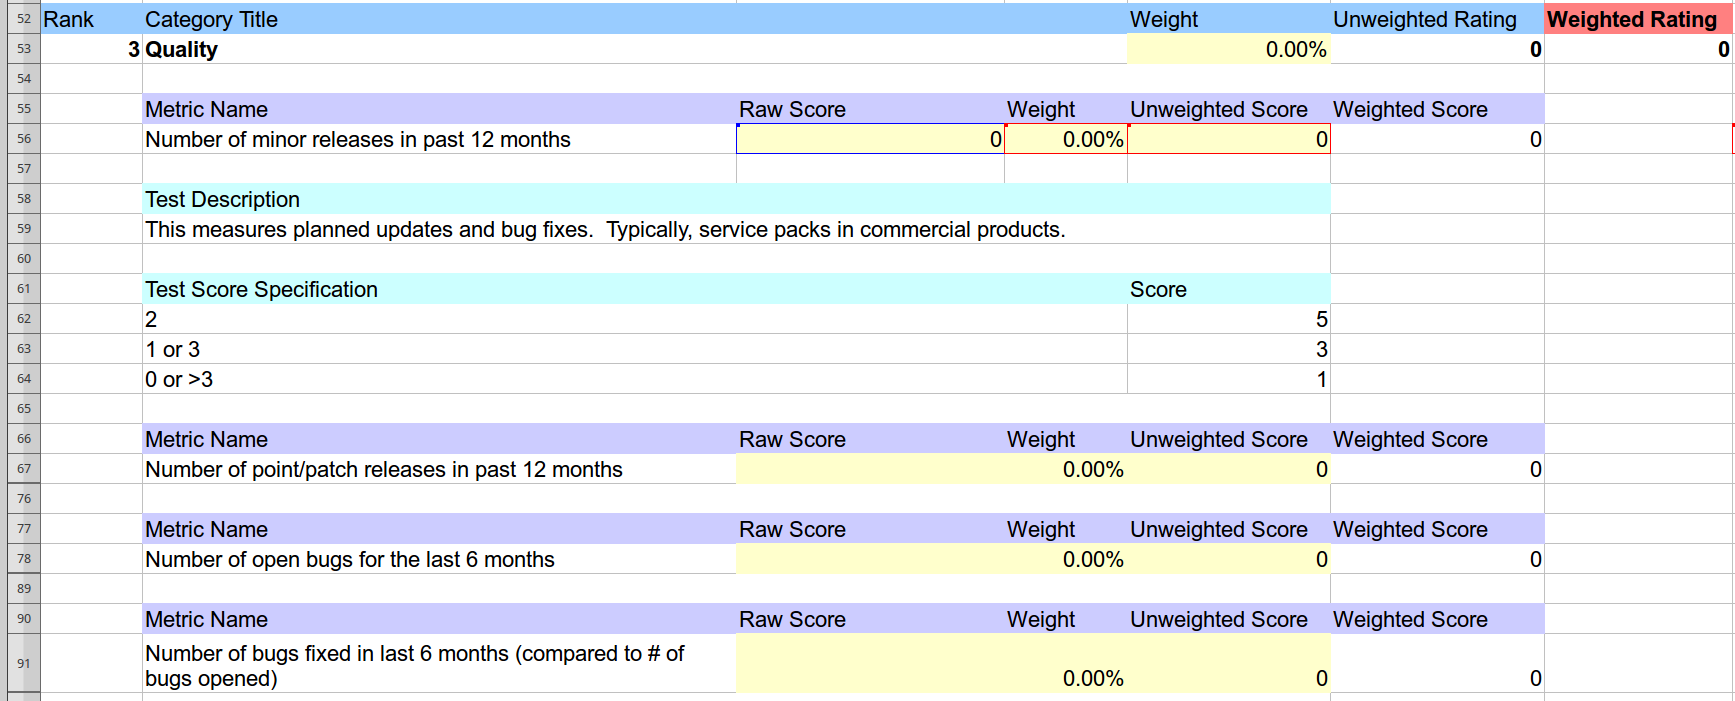
\includegraphics[width=16cm]{img/openbrr_extract00.png}
   \caption{Categoría OpenBRR}
   \label{fig:openbrrcategory}
 \end{center}
 \end{figure}
\end{center}

Las categorías que este modelo propone son las siguientes:
\begin{enumerate}
\item{\underline{Funcionalidad}}. Grado de cumplimiento de las funcionalidades requeridas.
\item{\underline{Usabilidad}}. Desde el punto de vista de experiencia de usuario, tiempos de instalación y configuración, etc.
\item{\underline{Calidad}}. Orientado a número de releases, parches, bugs críticos abiertos o tiempo de resolución de los mismos.
\item{\underline{Seguridad}}. Número de vulnerabilidades moderadas y/o críticas en determinados períodos de tiempo.
\item{\underline{Rendimiento}}. Disponibilidad de benchmarks, configuración de performance+tuning, etc.
\item{\underline{Escalabilidad}}. De forma que se establezca si el software está bien adaptado para ser escalado.
\item{\underline{Arquitectura}}. Se contemplan, dentro de esta categoría, aspectos como la existencia de plugins de terceros, o si se proporcionan APIs (Application Program Interface).
\item{\underline{Soporte}}. Se evalúan aspectos como la actividad en las listas de correo del proyecto, o la existencia de soporte profesional y su calidad.
\item{\underline{Documentación}}. Existencia de documentación variada, desde manuales de usuario, instalación, administración, despliegue o guías de desarrollo.
\item{\underline{Adopción}}. Esta categoría plantea la existencia de libros en torno al proyecto, o bien la existencia de una base de usuarios real medible.
\item{\underline{Comunidad}}. Aspectos como el número de contribuidores únicos de código en los últimos meses son los que se contemplan en esta categoría del modelo.
\item{\underline{Profesionalismo}}. En esta categoría se analizan aspectos como la existencia de un líder del proyecto o la dificultad que se presenta a la hora de entrar en el equipo de desarrollo.
\end{enumerate}

Como puede observarse en la descripción de las categorías, si bien este modelo no recoge métricas específicas del código fuente, la parte más interesante que presenta es la evaluación de las métricas que realiza, debido, básicamente, a tres aspectos:
\begin{enumerate}
\item{\underline{Sencillez}}. Este modelo plantea un modo muy sencillo de evaluación de las métricas basado en puntuación más ponderación de cada una de ellas.
\item{\underline{Flexibilidad}}. La posibilidad de ponderación de cada una de las categorías y subcategorías permite al usuario establecer qué métricas y conjuntos de métricas son las que tienen más impacto a la hora de evaluar la calidad.
\item{\underline{Extensibilidad}}. El planteamiento que permite este modelo y la fácil implementación de su evaluación permiten extender la evaluación mediante, simplemente, añadir o eliminar categorías o subcategorías según se establezca que es necesario para el usuario final.
\end{enumerate}

Por tanto, si bien OpenBRR no realiza un análisis de métricas de código fuente, su filosofía y la fácil implementación de métricas que el modelo propone pueden servir perfectamente en la evaluación del modelo de calidad del código fuente.

\item{\underline{QSOS}~\cite{qsos:qsos} (Qualification and Selection of Opensource Software)}. Modelo de calidad ligero cuya especificación se establece en el ``QSOS Manifesto''. Básicamente, este manifiesto establece una serie de puntos que definen el modelo de calidad, resumidos en los siguientes objetivos principales:
\begin{enumerate}
\item{Análisis de necesidades y limitaciones en la adopción del software}.
\item{Evaluación funcional y de requisitos técnicos}.
\item{Formalización de metodología}.
\item{Proporcionar un método libre y abierto}.
\end{enumerate}
Basado en dichos objetivos principales, QSoS define un proceso iterativo que consiste en cuatro puntos independientes para llevar a cabo el modelo de calidad.

Teniendo en cuenta que el objetivo de este documento no es realizar un análisis detallado de cada uno de los modelos de evaluación de calidad en proyectos Open Source, puede destacarse, de forma muy resumida, que si bien QSoS es considerado un modelo de evaluación ligero, su implementación es más complicada respecto a OpenBRR. Además, al igual que ocurría con OpenBRR, carece de métricas específicas de calidad de software desde el punto de vista del código fuente. Por tanto, este modelo de calidad no añade ninguna mejora respecto a lo ofrecido por OpenBRR.
\end{itemize}

\subsubsection{Modelos Pesados de Análisis de Calidad de proyectos Open Source}

Bajo este capítulo se expone, básicamente, el modelo QualOSS, modelo considerado como modelo pesado de evaluación de calidad en proyectos de Open Source.
\begin{itemize}
\item{\underline{QualOSS}~\cite{qualoss:qualoss} (Quality Of Open Source Software)}. Este modelo, fundado en 2006 y financiado principalmente por la unión europea, persiguió rellenar el hueco detectado en el estado del arte de los modelos de evaluación de calidad en proyectos Open Source.

Este método tiene como primera intención una automatización semi-completa del análisis de los proyectos y de la obtención de sus métricas, mediante la descarga a través de herramientas como FLOSS-metrics, junto a una serie de scripts que permitan la optimización de esta tarea.

La metodología utilizada por este proyecto consistía básicamente en:
\begin{enumerate}
\item{\underline{Pasos Iniciales}}. En la primera etapa, se realizaron una serie de entrevistas con compañías y se identificaron las prioridades de las mismas a la hora de incorporar el uso corporativo de algún proyecto Open Source.
\item{\underline{Modelo Básico de Calidad}}. Este modelo establece una metodología GQM(Goal - Question - Metric) donde cada objetivo se divide en diversas preguntas y diversas métricas resultantes de las preguntas.
\item{\underline{Consideraciones de la Comunidad}}. Finalmente, se establecen atributos indispensables desde el punto de vista de la comunidad, como el tamaño de la misma, la adecuación, la regeneración, carga de trabajo, etc.
\end{enumerate}
\end{itemize}

Como puede observarse, este método hace una especial incidencia en las métricas. Sin embargo, debido, entre otros factores, a la finalización del proyecto y la no disponibilidad de las métricas en cuestión que se plantearon, unido al hecho de que se trata de una metodología pesada, no se puede considerar QualOSS como un modelo del que se puedan aprovechar ciertas herramientas o planteamientos. Sin embargo, el carácter de automatización que plantea en torno a la obtención de métricas es, sin duda, otro factor importante que también debe ser tenido en cuenta. 

En esta sección se ha realizado un repaso de los modelos de calidad existentes en la evaluación de proyectos Open Source. Si bien los modelos de calidad no son directamente aplicables, debido al hecho de que carecen de métricas específicas de calidad en el código fuente, cabe destacar que para la implementación de un modelo de calidad de este tipo algunas de las características de los modelos anteriores son deseables:

\begin{enumerate}
\item{\underline{Sencillez}}. El modelo elegido debe ser sencillo en su aplicación. De esta forma, se podrá asegurar su utilización en un mayor número de entornos.
\item{\underline{Flexibilidad}}. La posibilidad de ponderación de cada una de las métricas elegidas, ya sea a través de una propuesta de categorías y subcategorías, en la forma en la que lo hace OpenBRR, y permitir al usuario establecer qué métricas y conjuntos de métricas son las que tienen más impacto a la hora de evaluar la calidad en la aplicación del modelo, es una característica muy recomendable a implementar en el modelo de calidad.
\item{\underline{Extensibilidad}}. El modelo propuesto debe permitir, de forma sencilla, ser extendido con métricas no contempladas. De esta forma, se favorecerá en el modelo la aplicación de cambios para extender el conjunto de categorías y subcategorías de métricas y su posterior evaluación.
\item{\underline{Automatización}}. Cabe destacar que, a la hora de implementar el modelo, es recomendable adecuar éste para poder automatizar la obtención de resultados. Si bien el modelo puede quedar planteado a través de una hoja de cálculo, sería deseable establecer un mini-framework de herramientas, a través de scripting o de la implementación de una suite de llamadas a herramientas, de forma que se pudiera automatizar la evaluación de la calidad cumpliendo las características anteriores.
\item{\underline{Iterativo e incremental}}. Además de las características anteriores, es deseable que el modelo planteado se ajuste a un enfoque iterativo e incremental. Basado en las facultades anteriores, como son la sencillez, la flexibilidad y la extensibilidad, el modelo planteado será modificado y extendido para tratar de conseguir un modelo cada vez más robusto.
\end{enumerate}

Una vez establecidas las características básicas del modelo, es deseable realizar un estudio de las principales métricas existentes en el análisis del código fuente, tanto desde el punto de vista del diseño orientado a objetos como desde el punto de vista de análisis de código funcional, para establecer en qué medida estas métricas afectan a la calidad y, de esta forma, evaluar el posible impacto de las métricas en el modelo elegido.

\subsection{Métricas de diseño orientado a objetos}

En el apartado de métricas de software orientado a objetos, cabe destacar que hay diversos aspectos a estudiar a la hora de establecer la calidad. A lo largo del tiempo, estas métricas se están usando de forma incremental tanto para evaluar como para predecir la calidad~\cite{oometrics:introduction}. Un gran número de resultados empíricos soportan la validez de estas métricas~\cite{validation:oodesignasqualityindicators}, y de forma habitual se usan como un indicador temprano de atributos a los que está relacionada la métrica, como puedan ser la robustez, la mantenibilidad o la propensión a fallos, ya que normalmente, éstos últimos, no pueden ser evaluados hasta una etapa muy tardía dentro del proceso de desarrollo software.

Las métricas descritas en este punto están tomadas del conjunto de métricas MOOD~\cite{mood:metricsset}. A continuación se exponen las diversas métricas a considerar:

\subsubsection{Acoplamiento}
En 1974, Stevens et. al definieron el acoplamiento como ``la medida de fuerza de asociación establecida por la conexión de un módulo a otro''~\cite{structuredesign:coupling}. Básicamente, el acoplamiento define la interdependencia entre dos objetos. Los objetos A y B están acoplados si un método del objeto A llama a un método del objeto B. Normalmente, un acoplamiento excesivo indica una encapsulación débil y puede afectar a la reutilización del módulo.

\subsubsection{Cohesión}
El concepto de cohesión se refiere a cuan relacionados están los métodos y atributos de una clase con respecto al resto, esto es, el grado en que los métodos están relacionados con las variables de una clase. El LOCOM (Lack of Cohesion) es una medida que establece el conjunto de métodos locales disjuntos entre sí.

La Cohesión puede medirse de varias formas. Un método para poder medir la cohesión es calcular qué porcentaje de métodos utiliza cada una de las variables y hacer una media de dichos porcentajes.

Una alta cohesión implica una buena subdivisión de clases, mientras que una baja cohesión incrementa la complejidad, aumentando la probabilidad de errores, y es, sin duda, indicativo de un mal diseño y de futuros problemas en la reusabilidad. Las clases poco cohesivas deben ser partidas en clases con más cohesión.

\subsubsection{Encapsulación}
La ocultación de información es un mecanismo de diseño que permite que únicamente un subconjunto de sus métodos sean conocidos por los usuarios del módulo. La ocultación de información da lugar a la encapsulación en los lenguajes orientados a objetos. Se considera que los programas con un buen nivel de encapsulación son más fáciles de modificar (hasta en un factor 4) respecto a los programas que no lo son \cite{improving:softwareproductivity}.

Básicamente, la encapsulación se proporciona a través de dos métricas:

\begin{itemize}
\item{\underline{AHF} (Attribute Hiding Factor)}. Referencia a la invisibilidad de los atributos de una clase para el resto de clases. Lo ideal es que este valor sea de un 100\% (las clases externas no pueden acceder a ningún atributo de la clase).
\item{\underline{MHF} (Method Hiding Factor)}. Referencia a la invisibilidad de los métodos de una clase para el resto de clases. La ocultación de métodos incrementa la reusabilidad de otras aplicaciones y reduce la complejidad.
\end{itemize}

\subsubsection{Herencia}
La herencia de objetos decrementa la complejidad a través de la reducción del número de operaciones, pero es un tipo de relación entre clases que puede complicar el diseño y el mantenimiento. Se utilizan básicamente dos métricas en torno a la herencia:

\begin{itemize}
\item{\underline{DIT} (Depth of Inheritance Tree)}. Se define como la profundidad máxima de una clase nodo (que no tiene más clases hijas) dentro del árbol jerárquico de herencia. Cuanto más profunda una clase dentro de una herencia de clases, mayor número de métodos y atributos hereda, haciendo más complejo su diseño, su mantenimiento y su propensión a errores. 
\item{\underline{NOC} (Number of Children)}. Esta métrica define directamente el número de subclases de una clase. Las clases que tienen un gran número de hijos se consideran difícil a la hora de modificar y se consideran más complejas y propensas a errores.
\end{itemize}

\subsubsection{Complejidad de clase}

El concepto de complejidad de clase viene directamente definido por la métrica WMC (Weighted Methods/Class). Este valor directamente enumera la cantidad de métodos que tiene una clase. 

A mayor número de métodos, mayor complejidad (siempre que se tenga un valor razonable que no haga que las clases sean clases perezosas).

Cabe destacar que, sin embargo, existen otras tendencias que establecen que es más recomendable tener un mayor número de métodos siempre y cuando estos sean sencillos~\cite{refactoring:improvingdesign}

\subsection{Métricas de calidad de código de paquetes de clases}

\subsubsection{Estabilidad}
Se conoce como estabilidad a aquella característica que define la dificultad que implica que un módulo de software cambie debido al uso que hacen otros módulos de él.~\cite{unclebob:stabilityandabstraction}
Para medir la estabilidad se establece una métrica opuesta, la inestabilidad, definida como:

\begin{equation}
I = \frac{Ce}{Ca + Ce}
\end{equation}

Donde:
\begin{itemize}
\item{\underline{Ca}}: Es el número de clases, fuera del paquete a evaluar, que tienen dependencia con clases del paquete a evaluar.
\item{\underline{Ce}}: Es el número de clases, dentro del paquete a evaluar, que tienen dependencia con clases externas del paquete a evaluar.
\end{itemize}

Hay que destacar que la inestabilidad no es una característica a evitar, ya que si todos los paquetes fueran estables, el código sería difícil de modificar, algo que no es deseable. Simplemente hay que establecer en qué medida una clase estable debe cumplir otras características, como la abstracción, según se verá a continuación.

\subsubsection{Abstracción}
Debido a principios como DIP (Dependency Inversion Principle)~\cite{unclebob:stabilityandabstraction}, se establece que ciertos paquetes tienen que proporcionar clases abstractas que permitan establecer la relación entre las clases de alto nivel y aquéllas sobre las que se apoyan y que implementan los detalles específicos.

Se define como la abstracción de un paquete a la relación existente entre el número de clases abstractas y el total de clases que contiene:

\begin{equation}
A = \frac{Abstract Classes}{Total Classes}
\end{equation}

Como se comentó anteriormente, la Abstracción y la Estabilidad están estrechamente ligadas, ya que es deseable que los paquetes estables sean cuanto más abstractos mejor.

\subsubsection{Principio de Abstracciones Estables}

Este principio establece que cuanto más estable es un paquete, mayor abstracción debe proporcionar. De esta forma, se establece una relación directa entre Abstracción e Inestabilidad, de forma que un paquete debe posicionarse en la recta principal que relaciona ambos términos. Así, existe una secuencia principal de relación entre ambos, así como la distancia de la que se encuentra un paquete respecto a dicho valor. 

\begin{equation}
D = \frac{(A+I-1)}{\sqrt(2)}
\end{equation}

Dicha distancia tiene un valor entre 0 y $\frac{1}{\sqrt(2)}$. Sin embargo, puede modificarse para dar un valor normalizado, conocido como D':

\begin{equation}
D' = |A+I-1|
\end{equation}

Si la distancia es cero, los paquetes pueden considerarse fácilmente reusables y modificables. Si un paquete se aleja del valor Distancia igual a cero, entonces el paquete debe ser reestructurado.

\subsection{Métricas de calidad de código fuente}

Este apartado recoge una serie de características relacionadas con el desarrollo de software desde el punto de vista de programación estructurada. 

\subsubsection{Código duplicado}

La duplicación de código es el enemigo número uno de un sistema bien diseñado. Representa trabajo adicional, riesgo adicional y complejidad innecesaria.~\cite{unclebob:cleancode}. El código duplicado debe ser modificado y refactorizado para evitar su duplicidad.

Si bien no existe una métrica específica, sí que debe asegurarse la no existencia de código duplicado dentro del software. Para ello deberán estudiarse las distintas herramientas que permitan detectar duplicidad en el código y establecer algún tipo de evaluación.

\subsubsection{Código muerto}
Se conoce como código muerto a aquél código existente que ya no se ejecuta por diversos motivos, tales como pueden ser cambios en diseño, condiciones que nunca se cumplen, etc. Este código todavía compila, pero es un ``mal olor del software''. Si se identifica, debe ser retirado, puesto que ``cuanto más tiempo esté, peor será su olor''~\cite{unclebob:cleancode}.

Si bien no se definen métricas específicas, sí que pueden establecerse, por ejemplo, métricas del tipo ``líneas de código muerto que tiene un software respecto al número total de líneas'' o similares.

\subsubsection{Número de parámetros por método}

Cuanto menor es el número de argumentos de una función, mejor es la comprensión de ésta, ya que los argumentos conllevan un esfuerzo comprensivo. Funciones de más de tres argumentos deben evitarse, y las que tienen más de tres deben ser evitadas o muy justificadas. La métrica es sencilla, puesto que a menor número de argumentos, mejor.

\subsubsection{Complejidad Ciclomática}

La Complejidad Ciclomática es un término acuñado por McCabe en 1976~\cite{mccabe:acomplexitymeasure}, que permite establecer la complejidad de un método a través de una cifra basándose en la complejidad del grafo resultante de los posibles flujos de control de dicho método.

Cuanto mayor complejidad ciclomática posee el código, menor será su mantenibilidad y más complejas serán las pruebas unitarias a realizar sobre el mismo. Es deseable que esta medida sea lo menor posible.

\subsubsection{Longitud de métodos}

Pese a que no hay una justificación razonable sobre la longitud que deben poseer los métodos, muchos autores, basados en su experiencia, recomiendan que cuanto menor sea la longitud de un método mejor será su comprensión y su mantenibilidad~\cite{unclebob:cleancode}.

Si bien un método no tiene porqué ser excesivamente complejo por ser muy largo (un método de 200 líneas puede, por ejemplo, tener complejidad ciclomática 1), parece razonable que se parta la funcionalidad de dicho código en métodos más pequeños para mejorar su legibilidad. Por tanto, el número de líneas de un método puede establecerse también como una métrica que posea un valor que cuanto menor sea, mejor.

\subsubsection{Formato de código fuente}

Hay que ser claro en el código fuente. Para ello, el formato de los ficheros de código fuente debe ser considerado como un factor importante, ``demasiado importante para ignorarlo o para no ser considerado religiosamente''~\cite{unclebob:cleancode}.
Respecto al formato que debe poseer el código fuente, resulta razonable que éste siga una serie de reglas para favorecer su legibilidad:

\begin{itemize}
\item{\underline{Longitud de fichero}}. Cuanto mayor es la longitud de un fichero mayor es la dificultad para entender su contenido\cite{unclebob:cleancode}. Existen recomendaciones que indican que más de 500 líneas de código por fichero empieza a ser poco recomendable. Sin embargo, existen herramientas como \textbf{cccc} que sugieren que la longitud de una clase no sea mayor de 2000 líneas, mientras que \textbf{Vera++} sugiere esta misma longitud como la longitud máxima de un fichero.
\item{\underline{Anchura de líneas de código}}. Tradicionalmente, la anchura de línea se limitaba a 80 (límite de Hollerith). Sin embargo, en la actualidad, con la anchura de los monitores actuales, anchuras de 100 y hasta 120 caracteres son razonables. Más de 120 caracteres de ancho empieza a ser ilegible.
\item{\underline{Nombrado}}. Se debe perseguir una correcta nomenclatura de las variables, clases y métodos. Deben perseguir un nombrado claro, que especifique de forma correcta el motivo de su existencia y clarifique la intención~\cite{unclebob:cleancode}. Nombres de variables con una única letra deben evitarse, más aún si son nombres que favorecen la confusión con números (i.e.: 'int l' ó 'int O', que pueden confundirse con los números 1 y 0 respectivamente). 
\item{\underline{Indentación}}. Se debe perseguir una correcta indentación del código fuente. Más allá del número de caracteres a usar, al menos se debe procurar no romper la indentación. También se encuentra desaconsejado el carácter tabulador, ya que se prefiere un número determinado de espacios en blanco.
\end{itemize}

\pagebreak

\section{Herramientas}

En el apartado anterior se han analizado algunas de las métricas más utilizadas a la hora de evaluar la calidad del software según diversos autores y métodos más o menos formales. Sin embargo, la medición de dichas métricas puede resultar ser de diversas complejidades, estar sujeta a distintos estados del arte en función de su madurez, etc.

Si bien no se desea realizar un estudio detallado de herramientas, este capítulo sí que pretende realizar un análisis superficial que permita establecer el cálculo de qué métricas de las anteriormente estudiadas pueden evaluarse, para, posteriormente, conocer cuáles de ellas pueden considerarse en el modelo de calidad.

Es deseable que las herramientas a analizar cumplan una serie de características:

\begin{itemize}
\item{\underline{Sencillez}}. El ámbito de este documento implica tener que realizar la evaluación de un modelo de calidad establecido que busca, entre otras características, la sencillez. Por tanto, es deseable que las herramientas a utilizar sobre las que se apoyará la evaluación de éste también lo sean.
\item{\underline{Open Source}}. El hecho de que las herramientas sean Open Source favorece el uso libre de la herramienta, así como la libertad de modificación favorece su extensibilidad y la facilidad de realizar mejoras, sobre todo en vistas a trabajos futuros.
\item{\underline{Automaticidad}}. Las herramientas utilizadas deben proporcionar mecanismos que favorezcan la automaticidad de su ejecución y de la extracción de los resultados.
\item{\underline{Sistema Operativo Linux}}. Debido a sus características, que favorecen la automaticidad por su potente línea de comandos así como la disponibilidad de herramientas de Open Source empaquetadas y su fácil instalación, es recomendable que las herramientas estén disponibles en el Sistema Operativo Linux.
\item{\underline{Lenguaje C++}}. Debido a los contenidos estudiados en la materia sobre la que versa este trabajo, el lenguaje requerido para el que se obtendrán las métricas deberá ser C++.
\end{itemize}

Una vez conocidas las características básicas que deben cumplir las herramientas, se van a analizar algunas de las más utilizadas dentro del análisis de métricas software.

\subsection{cccc}

cccc~\cite{metrictools:cccc} es una herramienta que permite calcular diversas métricas de software. Su funcionamiento es a través de la shell, lo que favorece su uso a la hora de automatizar su ejecución en un framework que lo contenga.

Respecto a las métricas que permite calcular que son de interés según lo comentado anteriormente, se encuentran:

\begin{itemize}
\item{\underline{LOC} (Lines of Code)}. Como medida básica, cccc permite extraer el número de líneas de código total, el número de líneas de código por clase o el número de líneas de código de cada método dentro de una clase.
\item{\underline{Complejidad Ciclomática}}. cccc permite evaluar la complejidad ciclomática total y por clase.
\item{\underline{WMC}}. La herramienta proporciona diversos valores de esta métrica, como son WMCv (número de funciones por otras clases) y WMC1 para el número total de funciones de una clase.
\item{\underline{DIT y NOC}}. La herramienta permite analizar, para una clase, la profundidad de su árbol de herencia y el número de hijos que tiene.
\item{\underline{CBO} (Coupling Between Objects)}. cccc proporciona el número de clases relacionados con una clase ya sea como cliente o como servidora.

\end{itemize}

En cuanto a la salida de las métricas, está disponible en formato .html, en formato .xml y en formato CSV. Por tanto, la extracción de las métricas puede ser analizada con una nueva herramienta de sencillo desarrollo.

La principal desventaja a la hora de utilizar esta herramienta es la no continuación de su desarrollo, puesto que parece que, lamentablemente, en 2013, su desarrollador principal dejó de mantenerla. Por tanto, para este trabajo, se han tenido que realizar parches a la herramienta, debido a distintos problemas detectados en la ejecución de la misma.

\subsection{cppdepend}

cppdepend~\cite{metrictools:cppdepend} es una herramienta comercial que permite calcular hasta más de 82 métricas de software. Es, por tanto, una solución muy buena para obtención de diversas métricas en un modelo de calidad. Como nota adicional, esta herramienta puede ser utilizada desde la shell, permitiendo esto una integración en tareas de automatización de obtención de métricas.

El principal problema que presenta es su naturaleza de software cerrado, que no permite extensiones. Además, su utilización no es simple, ya que precisa determinados ficheros "de proyecto" para obtener los ficheros que sirven como entrada a su generación. Su precio (499\$ en su versión más básica), tampoco la hace muy recomendable para el uso en el ámbito académico, aunque sí es una muy buena opción a la hora de utilizar en el mundo de la empresa.

Se trata, por tanto, de una solución a evitar en el caso en el que se puedan obtener métricas suficientes a través de otras herramientas.

\subsection{pmd / cpd}

Esta suite de herramientas~\cite{metrictools:pmdcpd} Open Source permite realizar análisis estático de código para detectar, básicamente, código muerto y código duplicado. Incluye ejecución desde comando, está disponible en Linux e incluye soporte para varios lenguajes de programación.

Mientras que la suite global, pmd, permite realizar detección de código muerto mediante detección de objetos no utilizados, cpd está más centrado en la detección de código duplicado.

Lamentablemente, la suite pmd no tiene reglas definidas para C++, aunque sí lo tiene cpd. Por tanto, esta herramienta puede utilizarse para la detección de código duplicado.

\subsection{cppcheck}

La herramienta cppcheck~\cite{metrictools:cppcheck} permite realizar análisis estático de código C++. Entre las distintas métricas, permite detectar errores de estilo o funciones que no se ejecutan nunca, lo que supone una métrica válida para analizar código muerto.

\subsection{Vera++}

La herramienta Open Source Vera++~\cite{metrictools:veraplusplus} permite verificar y analizar código fuente en el lenguaje de programación C++. Esta herramienta tiene definida una serie de reglas que permiten validad el formato del código. El análisis realizado por la herramienta es sobre todo relacionado con el formato del código, ya que comprueba, entre otras, la longitud de los ficheros, la anchura de las líneas o el nombrado de las variables.

La herramienta funciona en modo comando, y extender su funcionalidad a través de nuevas reglas o reprogramando las ya existentes es muy simple, lo que favorece su extensibilidad. A modo de ejemplo, para este trabajo, se han modificado los perfiles para ejecutar únicamente ciertas reglas y de esta forma evaluar únicamente las métricas descritas en el capítulo~\ref{sec:quality_model}.

\subsection{SonarQube}

SonarQube~\cite{metrictools:sonarqube} es una potente herramienta para la medición de calidad de un proyecto software. Posee plugins para varios lenguajes, entre ellos C++. Además, SonarQube permite utilizar diversas herramientas de obtención de métricas, como son cppcheck o Vera++ ó valgrind.

SonarQube es una herramienta desarrollada como Open Source, que permite ser extendida a través de plugins, y que tiene una gran base de usuarios. Entre las posibles desventajas de este software, básicamente se encuentra el hecho de que la curva de aprendizaje es algo más pronunciada comparada con las herramientas anteriores. Finalmente, comentar que si bien no posee comandos específicos de uso desde la shell para la lectura de resultados, el hecho de que utilice una base de datos permite automatizar la extracción de métricas, así como su análisis y clasificación.

Dicho lo anterior, cabe destacar que SonarQube, en relación al lenguaje de programación C++, actúa más como un framework de visualización que como una herramienta. Así, su uso está más relacionado con la visualización de datos que con la propia generación de métricas. En este trabajo se ha utilizado el API que proporciona SonarQube contra la herramienta Vera++ para analizar las métricas que ésta última proporciona.

\pagebreak

\section{Propuesta de Modelo de Calidad}
\label{sec:quality_model}

Una vez enumeradas las distintas herramientas disponibles, la funcionalidad que proporcionan y sus principales características, se ha realizado la siguiente propuesta de modelo de calidad. El enfoque seguido ha sido un enfoque iterativo e incremental, en el que para las primeras iteraciones se ha realizado un análisis de las métricas de manera manual a través de una única herramienta, que en este caso ha sido \textbf{cccc}.

Hay que destacar que, por facilidad a la hora de analizar los datos, algunos valores se han elegido de acuerdo a los valores propuestos por las herramientas. Por ejemplo, en el caso de la profundidad de jerarquía de herencia (DIT), la herramienta cccc avisa (WARNING) sobre valores mayores que 3 y menores o iguales a 6, y alerta (ERROR) sobre valores mayores o iguales a 7. De ahí que en la elección del modelo dichas cifras se hayan considerado como umbrales para cada uno de los valores. En todo caso, el peso de las métricas dentro de una categoría podrá variarse, al igual que se puede variar la ponderación de cada una de las categorías.

En posteriores iteraciones, se han ido incorporando herramientas que han permitido ampliar el modelo de calidad y, por tanto, hacer que éste sea más completo. Además, se han ido incluyendo herramientas de scripting para automatizar la ejecución de los comandos sobre el código fuente.

\subsection{Modelo de Calidad Propuesto}

Se ha establecido un modelo de calidad basado en tres distintas categorías para evaluar el código fuente. Dichas categorías son el Diseño Orientado a Objetos, la Calidad Estructural y la Calidad del Formato del Código. A continuación se propondrán las diversas tablas que especifican cada una de las categorías:

\begin{table}[H]
  \begin{center}
    \begin{tabular}{ | p{1.6cm} | p{3cm} | p{8cm} | p{2cm} | }
    \toprule
    \textbf{Métrica} & \textbf{Descripción} & \textbf{Especificación de Valoración} & \textbf{Valoración} \\
    \hline
    WMC1 & Número de métodos por clase & Ninguna clase posee más de 30 métodos & 5 \\ \cline{3-3} \cline{4-4} 
    & & Existen varias clases con más de 30 métodos pero ninguna con más de 100 métodos & 3 \\ \cline{3-3}\cline{4-4}
    & & Existen clases con más de 100 métodos & 0 \\ \cline{3-3}\cline{4-4}
    \hline
    WMCv & Número de métodos públicos por clase & Ninguna clase posee más de 10 métodos públicos & 5 \\ \cline{3-3} \cline{4-4} 
    & & Existen varias clases con más de 10 métodos públicos pero ninguna con más de 30 métodos públicos & 3 \\ \cline{3-3}\cline{4-4}
    & & Existen varias clases con más de 30 métodos públicos & 0 \\ \cline{3-3}\cline{4-4}
    \hline
    DIT & Profundidad de jerarquía en el árbol de herencia & Ninguna clase tiene una profundidad de jerarquía mayor que 3 & 5 \\ \cline{3-3} \cline{4-4} 
    & & Existen varias clases con una profundidad de jerarquía de más de 3, pero ninguna con profundidad mayor que 6 & 3 \\ \cline{3-3}\cline{4-4}
    & & Existen varias clases con una profundidad de jerarquía de más de 6  & 0 \\ \cline{3-3}\cline{4-4}
    \hline
    CBO & Acoplamiento entre objetos & Todas las clases tienen un acoplamiento menor o igual a 12 & 5 \\ \cline{3-3} \cline{4-4} 
    & & Varias clases tiene un acoplamiento mayor que 12 pero ninguna lo tiene mayor que 30 & 3 \\ \cline{3-3}\cline{4-4}
    & & Existen clases que tienen un acoplamiento mayor que 30 & 0 \\ 
    \bottomrule
    \end{tabular}
    \caption{Especificación de Métricas de Diseño Orientado a Objetos}
    \label{tab:metrics_ood}
  \end{center}
\end{table}

Cabe destacar que todas las métricas expuestas en la Tabla~\ref{tab:metrics_ood} pueden obtenerse a partir de la herramienta \textbf{cccc}.

\begin{table}[H]
  \begin{center}
    \begin{tabular}{ | p{1.6cm} | p{3cm} | p{8cm} | p{2cm} | }
    \toprule
    \textbf{Métrica} & \textbf{Descripción} & \textbf{Especificación de Valoración} & \textbf{Valoración} \\
    \hline
    LOC & Número de líneas por clase & Ninguna clase tiene más de 500 líneas de código & 5 \\ \cline{3-3} \cline{4-4} 
    & & Existen clases que tienen más de 500 líneas de código, pero ninguna de más de 2000 líneas & 3 \\ \cline{3-3}\cline{4-4}
    & & Existen clases con más de 2000 líneas de código & 0 \\ \cline{3-3}\cline{4-4}
    \hline
    McCC & Complejidad Ciclomática de McCabe & Ninguna clase posee un valor complejidad superior 200 & 5 \\ \cline{3-3} \cline{4-4} 
    & & Existen clases con complejidad mayor de 200 pero ninguna superior a 1000 & 3 \\ \cline{3-3}\cline{4-4}
    & & Existen clases con complejidad superior a 1000 & 0 \\ \cline{3-3}\cline{4-4}
    \hline
    DUP & Código Duplicado & No existe código duplicado de más de 100 tokens & 5 \\ \cline{3-3} \cline{4-4} 
    & & Existe Código Duplicado de entre 100 y 500 tokens & 3 \\ \cline{3-3}\cline{4-4}
    & & Existe Código Duplicado de entre 500 y 1000 tokens & 1 \\ \cline{3-3}\cline{4-4}
    & & Existe Código Duplicado de más de 1000 tokens & 0 \\ 
    \bottomrule
    \end{tabular}
    \caption{Categoría: Métricas de Calidad Estructural de Código Fuente}
    \label{tab:metrics_struct}
  \end{center}
\end{table}

En cuanto a las herramientas utilizadas para las métricas descritas en la Tabla~\ref{tab:metrics_struct}, se puede utilizar \textbf{cccc} para la obtención de métricas de número de líneas por clase y complejidad ciclomática de McCabe, mientras que para la detección de código duplicado se puede utilizar \textbf{cpd}, dentro de la suite de herramientas \textbf{pmd}.

\begin{table}[H]
  \begin{center}
    \begin{tabular}{ | p{1.6cm} | p{3cm} | p{8cm} | p{2cm} | }
    \toprule
    \textbf{Métrica} & \textbf{Descripción} & \textbf{Especificación de Valoración} & \textbf{Valoración} \\
    \hline
    HEI & Longitud de fichero en líneas de código & No existen ficheros con más de 2000 líneas & 5 \\ \cline{3-3} \cline{4-4}
    & & Existen ficheros con más de 2000 líneas, pero ninguno es mayor de 4000 líneas & 3 \\ \cline{3-3}\cline{4-4}
    & & Existen ficheros con más de 4000 líneas & 0 \\ \cline{3-3}\cline{4-4}
    \hline
    WID & Anchura de líneas de código & No existen ficheros con líneas más anchas de 100 caracteres & 5 \\ \cline{3-3} \cline{4-4} 
    & & Existen ficheros con líneas de más de 100 caracteres, pero ningún fichero con más de 120 & 3 \\ \cline{3-3}\cline{4-4}
    & & Existen ficheros con líneas de más de 120 caracteres & 0 \\ \cline{3-3}\cline{4-4}
    \hline
    TAB & No se deben utilizar tabuladores para indentar el código & No existe ningún tabulador indentando el código & 5 \\ \cline{3-3} \cline{4-4} 
    & & Existen tabuladores en la indentación del código & 0 \\ \cline{3-3} \cline{4-4}
    \hline
    VAR & No se deben utilizar nombres de variables 'l' u 'O' & No existe ninguna variable con la nomenclatura 'l' u 'O' & 5 \\ \cline{3-3} \cline{4-4} 
    & & Existen variables con la nomenclatura 'l' u 'O' & 0 \\ 
    \bottomrule
    \end{tabular}
    \caption{Categoría: Métricas de Calidad de Formato de Código Fuente}
    \label{tab:metrics_format}
  \end{center}
\end{table}

Finalmente, para las métricas de código descritas en la Tabla~\ref{tab:metrics_format} se puede utilizar la herramienta \textbf{Vera++}.

\pagebreak

\section{Un ejemplo práctico: MongoDB vs. RethinkDB vs. ArangoDB}
\label{sec:quality_comparison}

\subsection{Análisis de la calidad del código}

Esta sección permitirá concretar el modelo de calidad elegido sobre los proyectos inspeccionados. De esta forma, se realizará una comparativa entre diversos proyectos, de temática similar, en este caso, Bases de Datos de tipo NoSQL, que estén desarrollados en C++ y que cuenten con un número de líneas de código similar entre sí, con diferencias de no más de un orden de magnitud.

En esta ocasión, los proyectos elegidos han sido MongoDB (LOC=920K, LOC-C++=740K), RethinkDB (LOC=315K, LOC-C++=218K) y ArangoDB (LOC=3M, LOC-C++=1,8M). El modelo de calidad se aplicará únicamente sobre el código C++ del proyecto, ignorando otros lenguajes de programación o código que no pertenezca al proyecto, como puedan ser \emph{third parties}.

Respecto a las categorías propuestas en el modelo de calidad, no se han considerado valores de ponderación especiales para ninguna de ellas. Esto implica que las categorías ponderadas serán similares en el modelo de calidad, y por tanto la puntuación no se verá sometida a ajustes de ponderación. Sin embargo, hay que aclarar que los valores de ponderación deben ser considerados según los aspectos que considere el rol que evalúa los proyectos. Según los objetivos, puede ser más importante darle mayor peso a las métricas de una categoría particular, como puedan ser las métricas de Diseño Orientado a Objetos, por ejemplo. 

Así mismo, la ponderación de métricas será equivalente dentro de cada una de las categorías. Al igual que ocurre con éstas últimas, en la evaluación que haga cada rol en situaciones de evaluación de calidad, se deberán considerar aquellos aspectos que puedan hacer que una categoría sume más que otra y su ponderación sea mayor respecto a otras. Dicho esto, en esta evaluación no se ha considerado ninguna métrica con más ponderación interna en la categoría.

Como puede observarse en la evaluación de los proyectos que se mostrará a continuación, para los diferentes proyectos evaluados, el proyecto que más puntuación obtiene es RethinkDB, 2.39. En segundo lugar aparece el proyecto ArangoDB, con una puntuación de 1.5, mientras que MongoDB obtiene una puntuación de 1.25. En la Figura~\ref{fig:quality_comparison} se muestra la comparativa de puntuación de los proyectos según las diversas categorías:

\begin{center}
 \begin{figure}[H]
 \begin{center}
   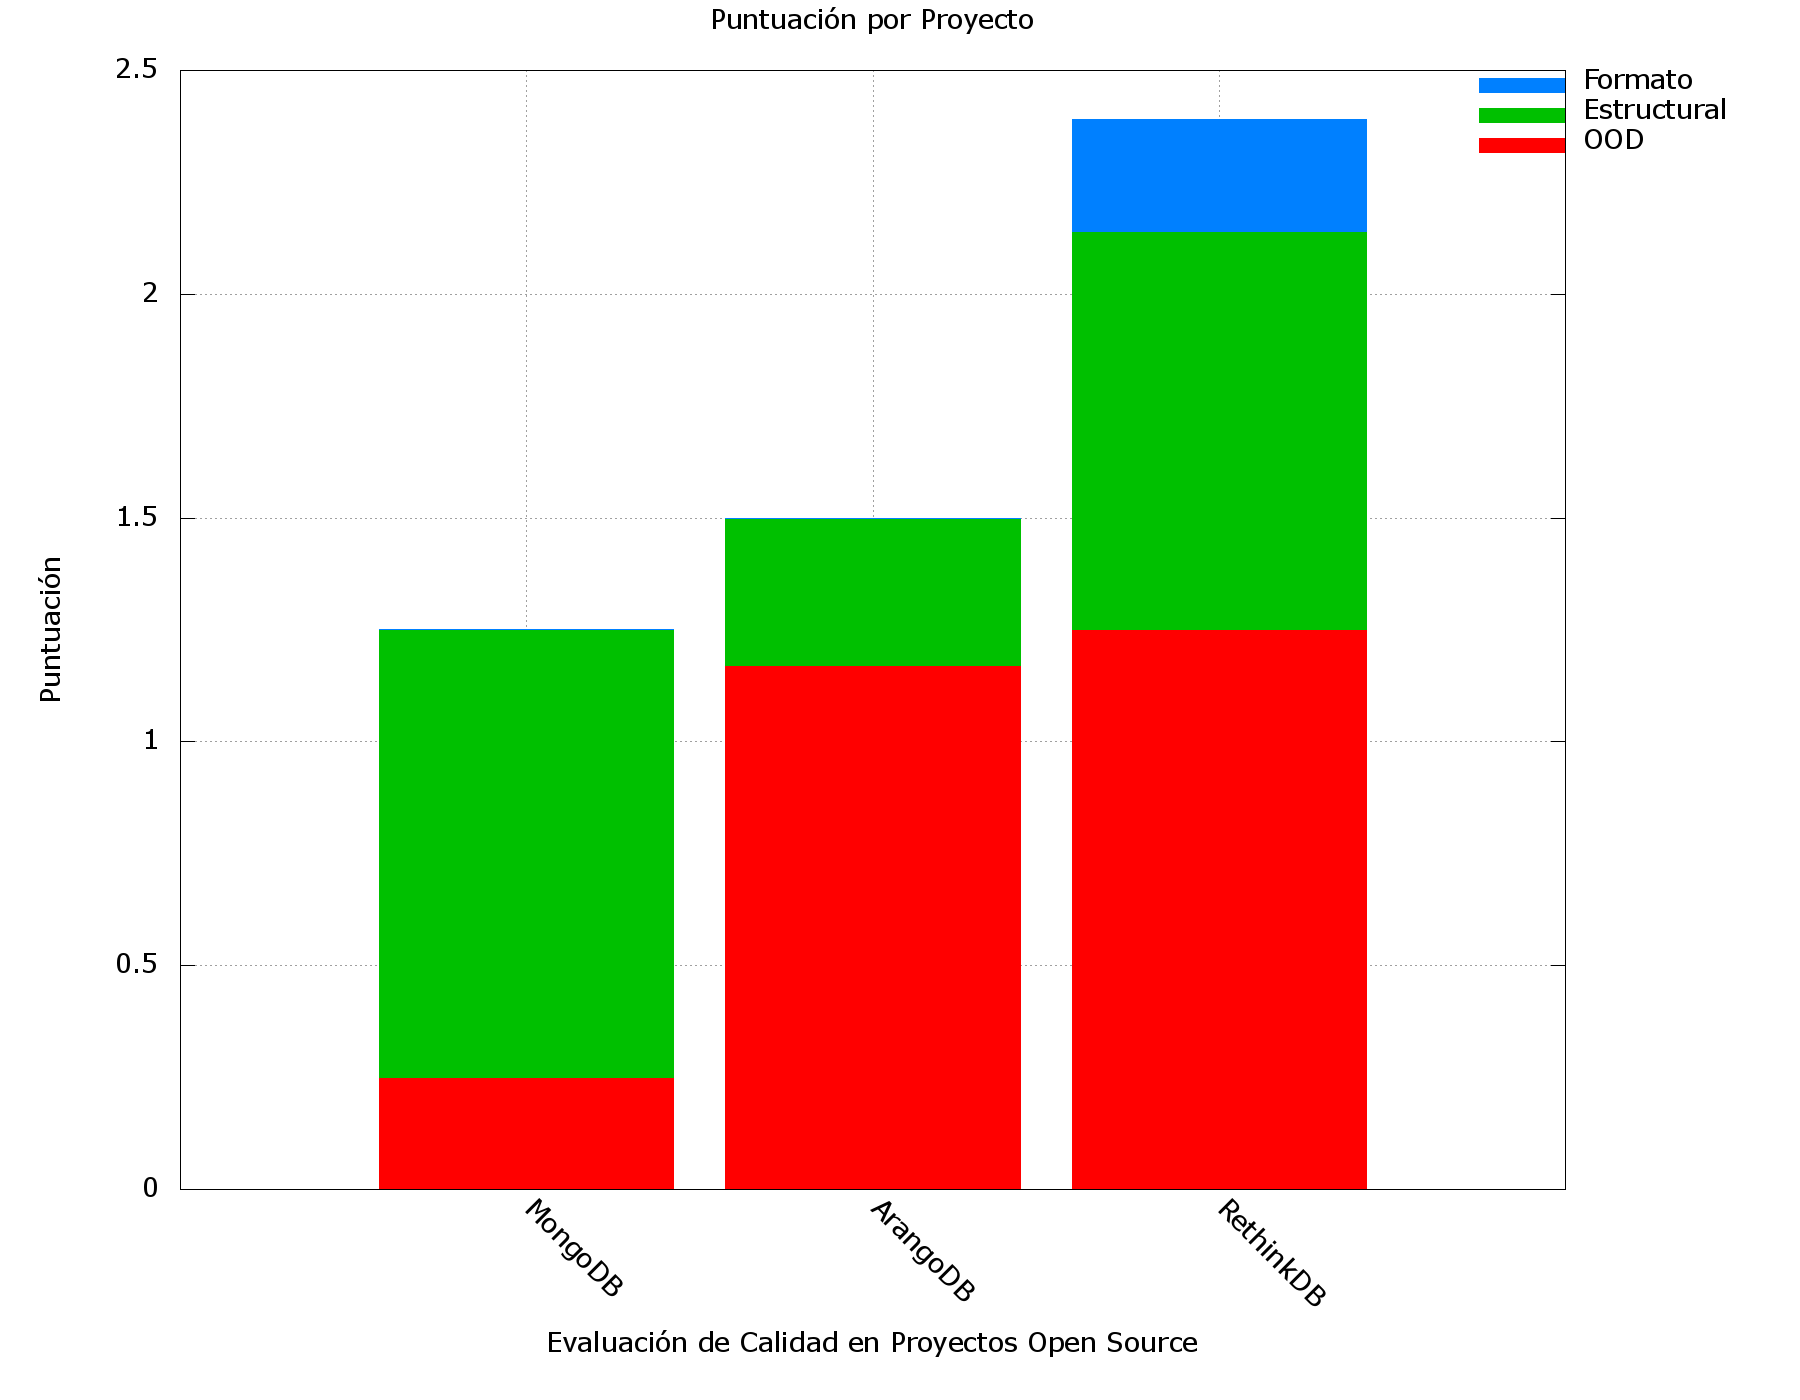
\includegraphics[width=16cm]{img/quality_evaluations.png}
   \caption{Comparativa de Calidad de Proyectos}
   \label{fig:quality_comparison}
 \end{center}
 \end{figure}
\end{center}

La puntuación de cada uno de los proyectos, clasificadas por categorías, junto a las métricas de cada una de éstas y la ponderación de las mismas es la que se muestra a continuación \footnote{Pueden descargarse las hojas de cálculo en GitHub: https://github.com/sarroutbi/TFE.git, directorio ``evaluation\_sheets'' }:

\begin{table}[H]
  \begin{center}
    \begin{tabular}{ | p{3.4cm} | p{5cm} | p {1cm} | p{2.3cm} | p{2.1cm} | }
    \toprule
    \multicolumn{5}{|c|}{\textbf{Métricas Orientación a Objetos}}\\
    \hline
    \textbf{Métrica} & \textbf{Valoración} & \textbf{Punt.} & \textbf{Pond. Métrica} & \textbf{Punt. Ponderada}\\
    \hline
    Nº métodos por clase & Varias con más de 30 métodos, ninguna por encima de 100 & 3 & 25\% & 0.75\\
    \hline
    Nº métodos públicos por clase & Varias clases con más de 10 métodos públicos, ninguna por encima de 30 & 3 & 25\% & 0.75\\
    \hline
    Profundidad en el árbol de herencia & Ninguna clase con profundidad mayor que 3 & 5 & 25\% & 1.25\\
    \hline
    Acoplamiento entre objetos & Varias clases tiene un acoplamiento mayor que 12 pero ninguna lo tiene mayor que 30 & 3 & 25\% & 0.75\\
    \midrule
    \textbf{Puntuación} & \multicolumn{4}{c|}{\textbf{3.5}}\\
    \hline
    \textbf{Puntuación ponderada (33.33\%)} & \multicolumn {4}{c|}{\textbf{1.17}}\\
    \midrule
    \multicolumn{5}{|c|}{\textbf{Métricas Estructurales}}\\
    \hline
    Número de Líneas por Clase & Existen clases con más de 2000 líneas de código & 0 & 33.33\% & 0\\
    \hline
    Complejidad Ciclomática & Existen clases con complejidad mayor de 200, pero ninguna mayor de 1000 & 3 & 33.33\% & 1\\
    \hline
    Código Duplicado & Existe código duplicado de más de 1000 tokens & 0 & 33.33\% & 0\\
    \midrule
    \textbf{Puntuación} & \multicolumn{4}{c|}{\textbf{1}}\\
    \hline
    \textbf{Puntuación ponderada (33.33\%)} & \multicolumn {4}{c|}{\textbf{0.33}}\\
    \midrule
    \multicolumn{5}{|c|}{\textbf{Métricas Formato de Código}}\\
    \hline
    Longitud de fichero en líneas de código & Existen ficheros con más de 4000 líneas & 0 & 25\% & 0\\ 
    \hline
    Anchura de líneas de código & Existen ficheros con anchura mayor a 120 & 0 & 25\% & 0\\
    \hline
    Existencia de tabuladores & Existe código indentado con tabuladores & 0 & 25\% & 0\\
    \hline
    Nombrado de variables & Existen variables con nombres como 'l' o 'O' & 0 & 25\% & 0\\
    \midrule
    \textbf{Puntuación} & \multicolumn{4}{c|}{\textbf{0}}\\
    \hline
    \textbf{Puntuación ponderada (33.33\%)} & \multicolumn {4}{c|}{\textbf{0}}\\   
    \midrule
    \multicolumn{5}{|c|}{\textbf{Puntuación total: 1.17 + 0.33 + 0 = \hl{1.5}}}\\
    \bottomrule
    \end{tabular}
    \caption{Puntuación Proyecto ArangoDB}
    \label{tab:arangodb_score}
  \end{center}
\end{table}

\begin{table}[H]
  \begin{center}
    \begin{tabular}{ | p{3.4cm} | p{5cm} | p {1cm} | p{2.3cm} | p{2.1cm} | }
    \toprule
    \multicolumn{5}{|c|}{\textbf{Métricas Orientación a Objetos}}\\
    \hline
    \textbf{Métrica} & \textbf{Valoración} & \textbf{Punt.} & \textbf{Pond. Métrica} & \textbf{Punt. Ponderada}\\
    \hline
    Nº métodos por clase & Existen clases con más de 100 métodos & 0 & 25\% & 0\\
    \hline
    Nº métodos públicos por clase & Existen clases con más de 30 métodos públicos & 0 & 25\% & 0\\
    \hline
    Profundidad en el árbol de herencia & Existen varias clases con una profundidad de jerarquía de más de 3, pero ninguna con profundidad mayor que 6 & 5 & 25\% & 0.75\\
    \hline
    Acoplamiento entre objetos & Existen clases que tienen un acoplamiento mayor que 30 & 0 & 25\% & 0\\
    \midrule
    \textbf{Puntuación} & \multicolumn{4}{c|}{\textbf{0.75}}\\
    \hline
    \textbf{Puntuación ponderada (33.33\%)} & \multicolumn {4}{c|}{\textbf{0.25}}\\
    \midrule
    \multicolumn{5}{|c|}{\textbf{Métricas Estructurales}}\\
    \hline
    Número de Líneas por Clase & Existen clases que tienen más de 500 líneas de código, pero ninguna de más de 2000 & 3 & 33.33\% & 1\\
    \hline
    Complejidad Ciclomática & Existen clases con complejidad mayor de 200, pero ninguna mayor de 1000 & 3 & 33.33\% & 1\\
    \hline
    Código Duplicado & Existe código duplicado de entre 100 y 500 tokens & 3 & 33.33\% & 1\\
    \midrule
    \textbf{Puntuación} & \multicolumn{4}{c|}{\textbf{3}}\\
    \hline
    \textbf{Puntuación ponderada (33.33\%)} & \multicolumn {4}{c|}{\textbf{1}}\\
    \midrule
    \multicolumn{5}{|c|}{\textbf{Métricas Formato de Código}}\\
    \hline
    Longitud de fichero en líneas de código & Existen ficheros con más de 4000 líneas & 0 & 25\% & 0\\ 
    \hline
    Anchura de líneas de código & Existen ficheros con anchura mayor a 120 & 0 & 25\% & 0\\
    \hline
    Existencia de tabuladores & Existe código indentado con tabuladores & 0 & 25\% & 0\\
    \hline
    Nombrado de variables & Existen variables con nombres como 'l' o 'O' & 0 & 25\% & 0\\
    \midrule
    \textbf{Puntuación} & \multicolumn{4}{c|}{\textbf{0}}\\
    \hline
    \textbf{Puntuación ponderada (33.33\%)} & \multicolumn {4}{c|}{\textbf{0}}\\   
    \midrule
    \multicolumn{5}{|c|}{\textbf{Puntuación total: 0.25 + 1 + 0 = \hl{1.25}}}\\
    \bottomrule
    \end{tabular}
    \caption{Puntuación Proyecto MongoDB}
    \label{tab:mongodb_score}
  \end{center}
\end{table}

\begin{table}[H]
  \begin{center}
    \begin{tabular}{ | p{3.4cm} | p{5cm} | p {1cm} | p{2.3cm} | p{2.1cm} | }
    \toprule
    \multicolumn{5}{|c|}{\textbf{Métricas Orientación a Objetos}}\\
    \hline
    \textbf{Métrica} & \textbf{Valoración} & \textbf{Punt.} & \textbf{Pond. Métrica} & \textbf{Punt. Ponderada}\\
    \hline
    Nº métodos por clase & Ninguna clase posee más de 30 métodos & 5 & 25\% & 1.25\\
    \hline
    Nº métodos públicos por clase & Ninguna clase posee más de 10 métodos públicos & 5 & 25\% & 1.25\\
    \hline
    Profundidad en el árbol de herencia & Ninguna clase posee una profundidad de jerarquía de más de 3 & 5 & 25\% & 1.25\\
    \hline
    Acoplamiento entre objetos & Existen clases que tienen un acoplamiento mayor que 30 & 0 & 25\% & 0\\
    \midrule
    \textbf{Puntuación} & \multicolumn{4}{c|}{\textbf{3.75}}\\
    \hline
    \textbf{Puntuación ponderada (33.33\%)} & \multicolumn {4}{c|}{\textbf{1.25}}\\
    \midrule
    \multicolumn{5}{|c|}{\textbf{Métricas Estructurales}}\\
    \hline
    Número de Líneas por Clase & Existen clases que tienen más de 500 líneas de código, pero ninguna de más de 2000 & 3 & 33.33\% & 1\\
    \hline
    Complejidad Ciclomática & Ninguna clase tiene complejidad mayor que 200 & 5 & 33.33\% & 1.67\\
    \hline
    Código Duplicado & Existe código duplicado de entre 100 y 500 tokens & 3 & 33.33\% & 1\\
    \midrule
    \textbf{Puntuación} & \multicolumn{4}{c|}{\textbf{3.67}}\\
    \hline
    \textbf{Puntuación ponderada (33.33\%)} & \multicolumn {4}{c|}{\textbf{1.22}}\\
    \midrule
    \multicolumn{5}{|c|}{\textbf{Métricas Formato de Código}}\\
    \hline
    Longitud de fichero en líneas de código & Existen ficheros con más de 2000 líneas, pero ninguno de más de 4000 líneas & 3 & 25\% & 0.75\\ 
    \hline
    Anchura de líneas de código & Existen ficheros con anchura mayor a 120 & 0 & 25\% & 0\\
    \hline
    Existencia de tabuladores & Existe código indentado con tabuladores & 0 & 25\% & 0\\
    \hline
    Nombrado de variables & Existen variables con nombres como 'l' o 'O' & 0 & 25\% & 0\\
    \midrule
    \textbf{Puntuación} & \multicolumn{4}{c|}{\textbf{0.75}}\\
    \hline
    \textbf{Puntuación ponderada (33.33\%)} & \multicolumn {4}{c|}{\textbf{0.25}}\\   
    \midrule
    \multicolumn{5}{|c|}{\textbf{Puntuación total: 1.25 + 1.22 + 0.25 = \hl{2.72}}}\\
    \bottomrule
    \end{tabular}
    \caption{Puntuación Proyecto RethinkDB}
    \label{tab:rethinkdb_score}
  \end{center}
\end{table}

\pagebreak

\section{Evaluación de histórico de calidad en el tiempo}
\label{sec:historic_quality}

Como se pudo apreciar en el capítulo~\ref{sec:quality_comparison}, un modelo de calidad puede servir para establecer unas pautas a la hora de evaluar la calidad y comparar entre diversos proyectos según unos parámetros de calidad basados en métricas previamente establecidos.

Sin embargo, este mismo modelo puede reaprovecharse para realizar el estudio de cómo ha sido la evolución de la calidad en un proyecto determinado, de forma que se pueda evaluar el progreso según el modelo planteado, y de esta forma revisar aquellos aspectos más relevantes a la hora de observar la progresión del proyecto en el tiempo, o, simplemente, observar cómo está siendo la evolución del proyecto en relación a los parámetros de calidad planteados.

Se ha realizado este ejercicio para los proyectos anteriormente mencionados, de forma que se han estudiado los valores de calidad del modelo en períodos anteriores de tiempo, en concreto hace uno y dos años, para ver cómo está siendo la evolución según el modelo establecido. Puede observarse en la tabla~\ref{tab:historic_quality} los resultados obtenidos \footnote{Pueden descargarse las hojas de cálculo en GitHub: https://github.com/sarroutbi/TFE.git, directorio ``evaluation\_sheets''}.

\begin{table}[H]
  \begin{center}
    \begin{tabular}{ | p{2cm} | p{2cm} | p{2cm} | p {2cm} | p{2cm} | p{2cm} | }
    \toprule
    \multicolumn{6}{|c|}{\textbf{Evaluación Histórica Proyecto ArangoDB}}\\
    \hline
    \textbf{Proyecto} & \textbf{Fecha} & \textbf{Punt. OO.} & \textbf{Punt. Est.} & \textbf{Punt. Form.} & \textbf{Punt. Pond.}\\
     \hline
     ArangoDB & Enero 2016 & 1.17 & 0.33 & 0 & \textbf{1.5}\\
     \hline
     ArangoDB & Enero 2015 & 1.17 & 0.78 & 0 & \textbf{1.94}\\
     \hline
     ArangoDB & Enero 2014 & 1.33 & 0.78 & 0 & \textbf{2.11}\\
     \hline
     \midrule
     \multicolumn{6}{|c|}{\textbf{Evaluación Histórica Proyecto MongoDB}}\\
     \hline
     \textbf{Proyecto} & \textbf{Fecha} & \textbf{Punt. OO.} & \textbf{Punt. Est.} & \textbf{Punt. Form.} & \textbf{Punt. Pond.}\\
     \hline
     MongoDB & Enero 2016 & 0.25 & 1 & 0 & \textbf{1.25}\\
     \hline
     MongoDB & Enero 2015 & 0.25 & 0.44 & 0 & \textbf{0.69}\\
     \hline
     MongoDB & Enero 2014 & 0.5 & 0.78 & 0 & \textbf{1.28}\\
     \hline
     \midrule
     \multicolumn{6}{|c|}{\textbf{Evaluación Histórica Proyecto RethinkDB}}\\
     \hline
     \textbf{Proyecto} & \textbf{Fecha} & \textbf{Punt. OO.} & \textbf{Punt. Est.} & \textbf{Punt. Form.} & \textbf{Punt. Pond.}\\
     \hline
     RethinkDB & Enero 2016 & 1.25 & 1.22 & 0.25 & \textbf{2.72}\\
     \hline
     RethinkDB & Enero 2015 & 1.25 & 1 & 0.25 & \textbf{2.5}\\
     \hline
     RethinkDB & Enero 2014 & 1.08 & 1.22 & 0.42 & \textbf{2.72}\\
    \bottomrule
    \end{tabular}
    \caption{Evaluación de Histórico de Calidad en el Tiempo}
    \label{tab:historic_quality}
  \end{center}
\end{table}

Según se observa en la figura~\ref{fig:quality_progression}, el proyecto ArangoDB ha ido decrementando, de forma gradual en el tiempo, la calidad en función del modelo planteado, lo que supone una mala progresión en base a las métricas definidas, lo que puede significar una desatención dentro del proyecto a aquellos aspectos que dicho modelo considera importantes. Mientras, para el proyecto MongoDB, se observa que, pese a que hace un año tuvo un decremento considerable, coincidiendo con una fuerte reestructuración de la base de código, al menos, se han conseguido recuperar los parámetros de calidad de los que se disponía hace dos años. Finalmente, en lo relativo al proyecto RethinkDB, parece que los parámetros de calidad han estado siempre por encima de los otros proyectos históricamente, y no se ha producido ninguna variación considerable en el histórico de tiempo analizado.

\begin{center}
 \begin{figure}[H]
 \begin{center}
   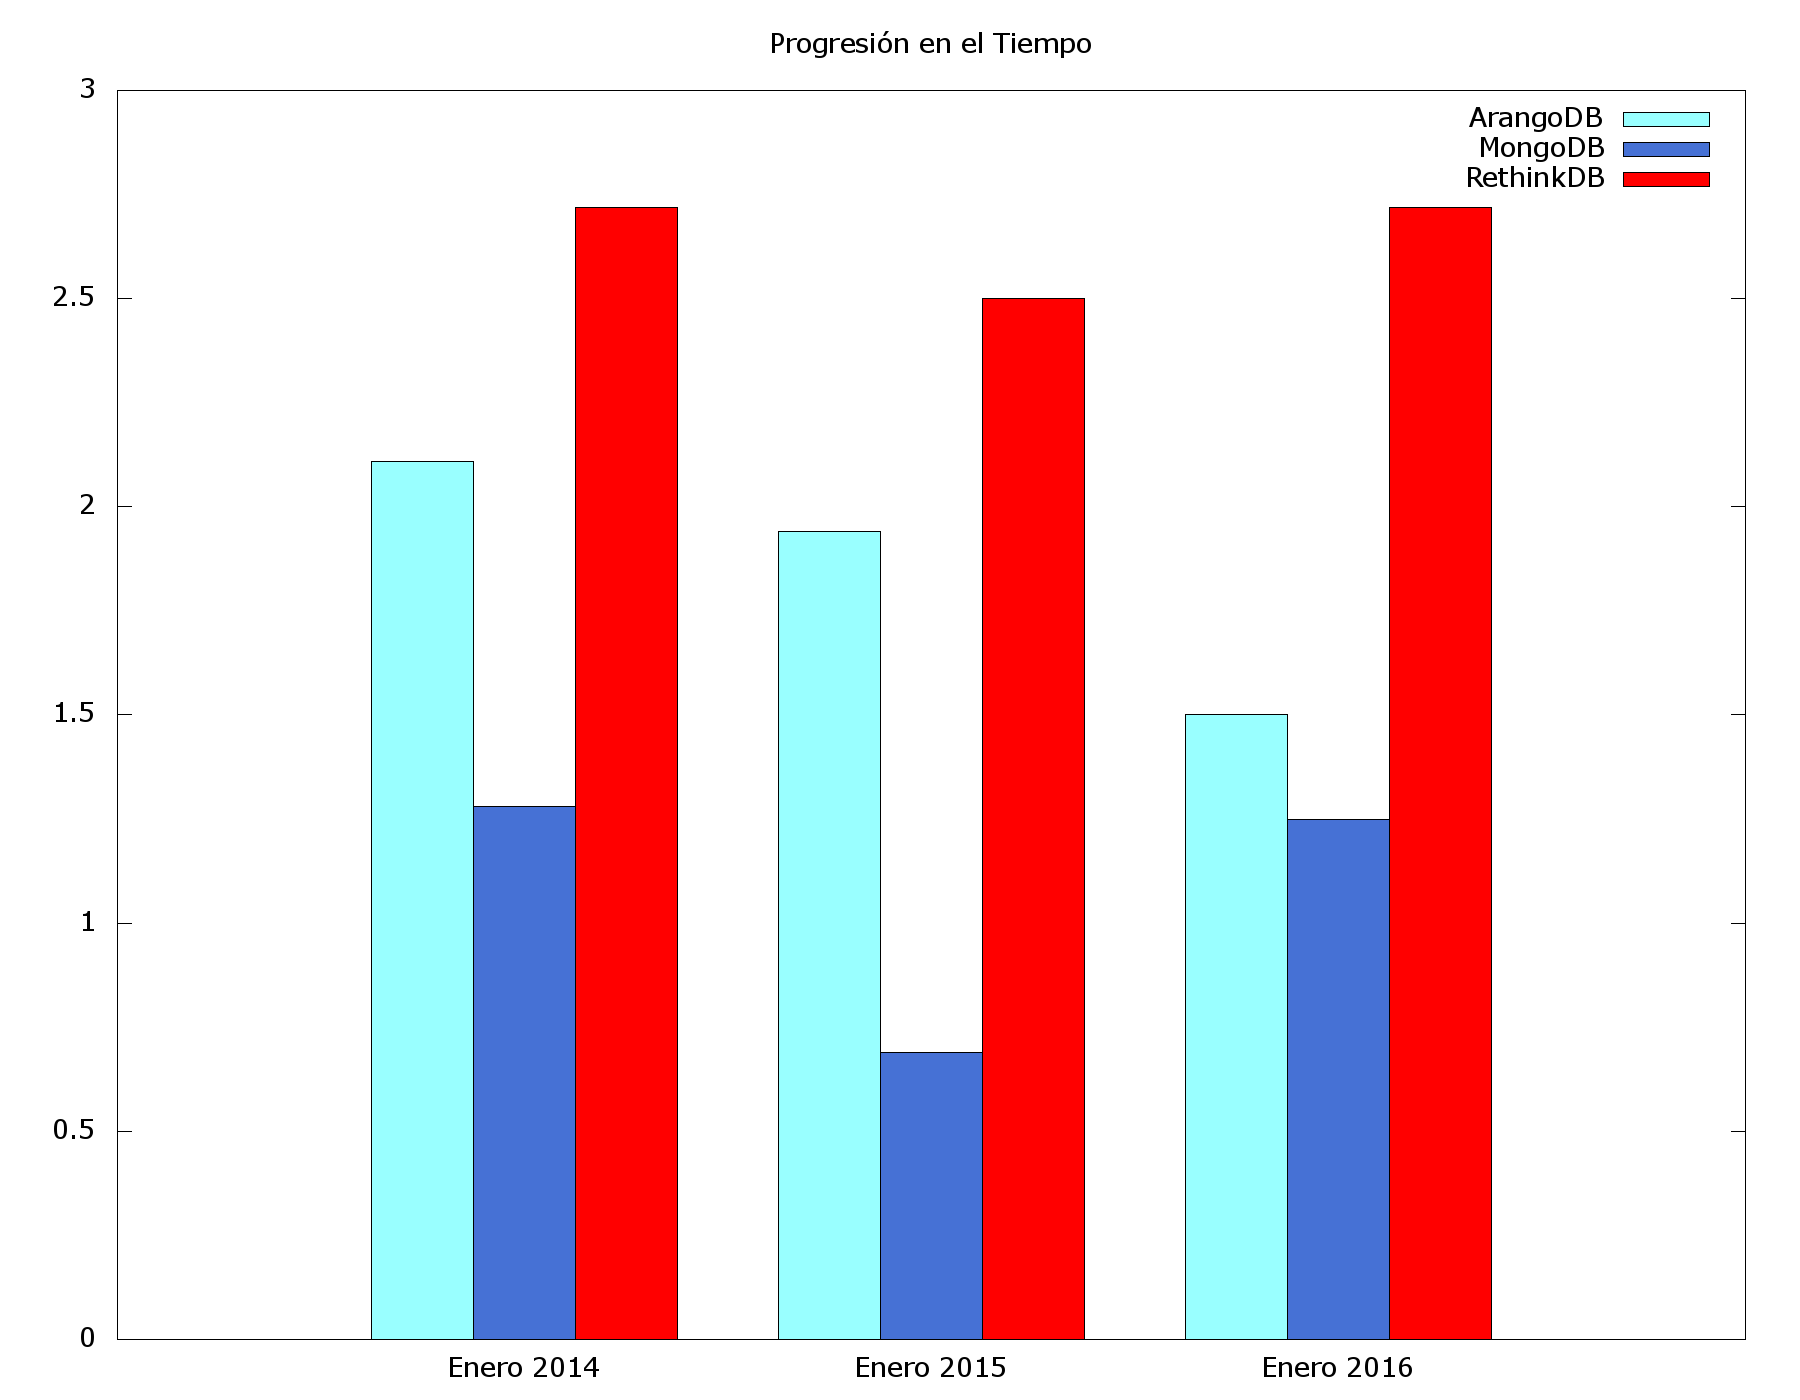
\includegraphics[width=16cm]{img/quality_progress.png}
   \caption{Comparativa de Histórico de Calidad}
   \label{fig:quality_progression}
 \end{center}
 \end{figure}
\end{center}

\pagebreak

\section{Conclusiones}
\label{sec:conclussions}

La calidad del código fuente importa. Es clave para un proyecto de software que el código cumpla unos requisitos de calidad establecidos. Esta importancia se acentúa a la hora de evaluar proyectos Open Source, debido a la transparencia que supone la naturaleza de este tipo de proyectos, que por definición deben hacer que su código fuente sea accesible.

A la hora de evaluar proyectos Open Source, la decisión de adquisición de alguna solución debe llevar asociado un estudio de la calidad del código fuente unido al modelo de calidad utilizado. Establecer modelos de calidad basados en métricas debe afrontarse como un ejercicio primordial en el desarrollo y/o evaluación de proyectos Open Source, y su evaluación durante el proceso de desarrollo debe llevarse a cabo de forma iterativa para detectar posibles riesgos, estudiar medidas de contingencia e integrar un proceso de mejora continua en el código fuente.

La existencia de las herramientas que han sido enumeradas en este documento permite acelerar la definición de modelos de calidad de software, pero es también imprescindible analizar las condiciones particulares de cada proyecto para establecer las métricas particulares, las preferencias de métricas para establecer las ponderaciones apropiadas y de esta forma adecuar su impacto en la calidad final.

\section{Mejoras y posibles trabajos futuros}

Como posibles mejoras se han identificado una serie de acciones que se pueden llevar a cabo para extender el trabajo anteriormente descrito:
\begin{enumerate}
\item{\underline{Modificación de herramientas para extracción de métricas}}. La utilización de herramientas de tipo Open Source abre la puerta a la extensión y/o mejora de éstas. Por ejemplo, se podría estudiar la extensión de \textbf{cccc} para hacer configurables los valores de ciertas métricas, ya que algunas de ellas son demasiado permisivas, como puede ser el número de métodos por clase. También se podría extender el tipo de métricas que esta herramienta proporciona.
Igualmente, cabe la posibilidad de extender la herramienta \textbf{Vera++} para incluir nuevas métricas de formato de código, como pueda ser la utilización de variables de menos de N letras, y no ceñirse únicamente a la evaluación de nombres confusos.
\item{\underline{Extensión del modelo de calidad}}. En otro orden de cosas, como mejora adicional, podría extenderse el modelo de calidad con más categorías y/o más métricas por categoría, mediante la utilización de otras herramientas no contempladas en este documento, o bien a través de las modificaciones enumeradas en el punto anterior.
\item{\underline{Automatización}}. Finalmente, pese a que para la selección de las herramientas se ha considerado la facilidad de uso de éstas para permitir la automatización de la extracción de las métricas, no se ha realizado dicha automatización como parte de este proyecto. Se propone, por tanto, como posible mejora, la realización de un framework que automatice total o parcialmente la obtención de las métricas y la generación de las puntuaciones del modelo de calidad.
\end{enumerate}

\pagebreak

\bibliographystyle{alpha}
\bibliography{bibliography}
\label{Bibliography}

\end{document}
 
